% paper.tex — anonymised single-column draft for IJBET (no journal name/logo/authors).
% Compile: pdflatex paper + biber paper + pdflatex paper + pdflatex paper
\documentclass[a4paper,11pt,en,citestyle=authoryear,bibstyle=authoryear]{elegantpaper}

\title{Calibrated Compact CNNs under Clinical Corruptions: Reliability of Lightweight Models on BloodMNIST and DermaMNIST}
\author{Author Name}
\institute{University Name}
\date{}

\addbibresource{references.bib}
\usepackage{microtype}
\usepackage{float}
\usepackage{tikz}
\usetikzlibrary{arrows.meta,positioning,fit,backgrounds}
\hypersetup{pdfauthor={}, pdftitle={Calibrated Compact CNNs under Clinical Corruptions}}

\begin{document}
\maketitle

\begin{abstract}
Blood-cell and skin-lesion classifiers are usually scored on clean accuracy, which is silent about confidence once inputs degrade. We trained compact networks on BloodMNIST and DermaMNIST with cross-entropy, focal and dual-focal losses over three seeds, fitted temperature scaling on the validation split, and measured accuracy, expected calibration error, negative log-likelihood, Brier score, AUROC, macro-F1 and balanced accuracy across eight corruptions at five severities. Scaling cut clean ECE roughly in half on blood (96.6\% accuracy, 0.7\% ECE) and by two thirds on skin lesions (76.5\% accuracy, 2.0\% ECE). The three losses separate once inputs are corrupted: dual-focal halves raw ECE before scaling, and after scaling all three sit near 0.7\% on blood. Shot noise breaks blood accuracy at severity 1 while confidence holds. Spatter densities inherited from 224-pixel benchmarks black out $28\times28$ frames, a failure we diagnose and correct by area scaling; even corrected, blood gives way by severity 3 where derma does not. A macro-F1 of 0.50 beside 76.5\% accuracy on derma is the clearest case we found for scoring these models on more than accuracy.
\keywords{Calibration, Medical Imaging, Robustness, Reliability Diagrams, Expected Calibration Error, Distribution Shift, BloodMNIST, DermaMNIST, Convolutional Neural Networks, Temperature Scaling, Uncertainty Quantification}
\end{abstract}

\section{Introduction}
A model that scores 96\% and remains certain when it is wrong will hurt somebody. In a clinic the confidence printed beside a prediction is read as advice, whether the reader is a clinician weighing a screening result or a technician deciding which slide needs a second look. Advice that is right 98\% of the time is worth acting on. Advice emitted at 98\% confidence while the model is guessing is worse than no advice at all, because it discourages the second look. Small-image benchmarks rarely test which of these two situations holds.

Calibration is the term for that honesty. A calibrated model gets about 80 of its 100 predictions right when it claims 80\% confidence. Weather forecasters had the idea well before deep learning did. Neural networks acquired a reputation for breaking it: training pushes them towards accuracy, and the confidence numbers drift upward whether or not the accuracy follows. On a clean test set that mirrors the training distribution the drift goes unnoticed. It becomes impossible to ignore when inputs degrade through noise, blur, a change in illumination or compression, which is the ordinary condition of a microscope or dermatoscope that has moved between rooms, operators and devices.

The MedMNIST collection standardised lightweight biomedical classification across modalities and scales \parencite{medmnist2023}, extending the classification decathlon that preceded it \parencite{medmnist2021}. Its corruption offshoot MedMNIST-C added distribution shift with accuracy-only scoring \parencite{medmnistc2024}, and no calibration figures have since been published on it. Ovadia and colleagues showed that post-hoc calibration falls short under shift on natural images \parencite{ovadia2019}; Minderer and colleagues found architecture to dominate calibration behaviour across 180 models \parencite{minderer2021}. Whether either observation survives the move to small clinical images was untested. We test it on two sets, BloodMNIST with 17,092 microscope cell images and DermaMNIST with 10,015 dermatoscopic skin lesion images.

Three questions drive the work. How do compact networks trained under different losses behave across corruption types and severities, both before and after temperature scaling? Which corruptions cost accuracy first, and which cost confidence first? And where does a corruption protocol built for $224$-pixel photographs stop making sense on a $28\times28$ frame? We answer from full training runs on a single Colab T4 GPU, with fixed seeds, the public splits and saved checkpoints, and with wider coverage of losses, seeds and metrics than earlier studies of this data.

Specifically, we report fixed-seed accuracy and calibration for three losses on two clinical sets across eight corruptions at five severities. We find that temperature scaling closes most of the gap between losses while raw calibration still favours dual-focal. We diagnose a protocol failure in spatter densities at $28\times28$, give the pixel-level evidence for it, and scale blob counts by image area to repair it. We add imbalance-aware metrics, which show accuracy alone misleading on skin lesions. Section~2 reviews the calibration and benchmark literature, Section~3 defines the metrics and losses, Section~4 sets out the datasets and protocol, Section~5 reports results, Section~6 discusses what they mean in practice, and Section~7 concludes.

\section{Related Work}
\subsection{Calibration}
The calibration literature starts with forecasters rather than networks. DeGroot and Fienberg formalised what it means for a stated probability to be honest \parencite{degroot1983}, and Brier gave the bounded score that still carries his name \parencite{brier1950}. Niculescu-Mizil and Caruana carried the question over to classifiers and found the small networks of their era calibrated well \parencite{nmic2005}. Naeini and colleagues replaced any single binning with an average over binnings \parencite{naeini2015}; Platt scaling fitted a logistic map on validation outputs \parencite{platt1999}. Guo and colleagues then showed that depth, width, batch normalisation and weak weight decay all degrade calibration while improving accuracy, and that one temperature parameter undoes most of the damage \parencite{guo2017}. Kumar and colleagues demonstrated that published calibration errors are systematically underestimated, and proposed a scaling-binning calibrator with an error bound \parencite{kumar2019}. Nixon and colleagues showed that the ranking of recalibration methods changes with the metric, and recommended class conditioning with adaptive bins \parencite{nixon2019}. Focal loss addressed calibration during training instead \parencite{focal2020}, and dual focal corrected focal's treatment of easy examples \parencite{dualfocal2023}. Ensembles \parencite{lakshminarayanan2017} and MC dropout \parencite{gal2016} marginalise over predictions rather than rescaling a single one, and Ovadia and colleagues found both outperform temperature scaling under strong shift \parencite{ovadia2019}. Our contribution continues that line on corrupted clinical images, holding losses fixed across seeds. Ensembles and dropout are not evaluated here.
\subsection{Medical Uncertainty and Benchmarks}
Leibig and colleagues estimated diabetic-retinopathy uncertainty with MC dropout and tied high uncertainty to wrong predictions \parencite{leibig2017}; that study remains the closest clinical analogue to our protocol. Hendrycks and Dietterich made distribution shift measurable with fixed corruptions and severities \parencite{corrupt2019}. MedMNIST v2 made lightweight clinical classification comparable across twelve 2D sets with frozen splits \parencite{medmnist2023}, and MedMNIST-C ported the corruption idea to those sets with modality-specific damage and accuracy-only scoring \parencite{medmnistc2024}. Calibration under that damage, with loss ablations, seed repeats and imbalance-aware metrics, had not been reported. The measurements below fill that gap for two of the twelve sets.

\section{Background and Notation}
Inputs $X$ take labels $Y \in \{1, \dots, K\}$. A network outputs logits $\mathbf{z}$ and probabilities $q = \sigma_{\mathrm{SM}}(\mathbf{z})$. Let $q_{gt}$ be the probability of the true class and $\hat{y} = \arg\max_k q_k$ the prediction with confidence $\hat{p} = \max_k q_k$. Perfect calibration means $\mathbb{P}(\hat{Y}=Y \mid \hat{P}=p) = p$ for all $p$. Finite samples force binning: group confidences into $M=15$ equal bins $B_m$ with accuracy $\mathrm{acc}(B_m)$ and mean confidence $\mathrm{conf}(B_m)$. A reliability diagram plots one against the other and the diagonal means calibrated. Expected calibration error compresses it \parencite{naeini2015}:
\begin{equation}
\mathrm{ECE} = \sum_{m=1}^{M} \frac{|B_m|}{n}\,\bigl|\mathrm{acc}(B_m)-\mathrm{conf}(B_m)\bigr|.
\end{equation}
NLL is unbounded and punishes confident errors without ceiling. Brier score \parencite{brier1950}:
\begin{equation}
\mathrm{Brier} = \frac{1}{n}\sum_{i=1}^{n}\sum_{k=1}^{K}(q_{ik} - y_{ik})^2,
\end{equation}
ranges 0 to 2 for multi-class problems, so values above 1.0 signal confident wrongness, not a bug. Classwise ECE averages one-vs-rest ECE over classes, which matters for imbalanced sets \parencite{nixon2019}.

Focal loss down-weights easy samples \parencite{focal2020}:
\begin{equation}
\mathcal{L}_{\mathrm{FL}} = -(1-q_{gt})^\gamma \log q_{gt}, \quad \gamma = 2.0.
\end{equation}
Dual focal loss widens the gap between the top two logits \parencite{dualfocal2023}. With $q_j$ the largest non-ground-truth probability:
\begin{equation}
\mathcal{L}_{\mathrm{DFL}} = -(1 - q_{gt} + q_j)^\gamma \log q_{gt}, \quad \gamma = 2.0.
\end{equation}
Temperature scaling divides every logit by one scalar $T>0$ fitted on validation NLL \parencite{guo2017}. It cannot change predictions, only confidence.

\section{Datasets and Protocol}
BloodMNIST provides 17,092 microscope cell images in eight classes, split 11,959/1,712/3,421 \parencite{acevedo2020}; DermaMNIST provides 10,015 dermatoscopic lesion images in seven classes, split 7,007/1,003/2,005 \parencite{tschandl2018}. Both are $28\times28$ RGB with frozen public splits (Table~\ref{tab:data}). One caveat travels with the second dataset: HAM10000 holds several images per lesion, so lesion-level leakage between its splits cannot be excluded. MedMNIST ships image-level splits, and we keep them.

Eight corruptions are applied to test images at severities 1--5, using the sample index as the seed so that every configuration faces identical damage and noise draws correlate across corruption types by construction. All operations run on 0--255 uint8 images before normalisation, with nearest-neighbour downsampling for pixelation, PIL quality settings for JPEG, and Gaussian blur radius in pixels (Table~\ref{tab:corr}). Because noise is injected after downsampling to $28\times28$, it overstates real sensor damage, which occurs at native resolution and partly averages away; severities are therefore comparable within a corruption type but not across types. One consequence matters downstream: shot noise at severity 1 already matches Gaussian noise at severity 5 in damage.

ResNet-18 uses a $3\times3$ stride-1 stem with no early max-pooling and has 11.17M parameters. SimpleCNN stacks three convolutional blocks in 0.14M parameters and is the genuinely lightweight arm of the two; ResNet-18 is mid-sized, and we name it as such throughout. Training uses AdamW \parencite{loshchilov2019} at learning rate $10^{-3}$ and weight decay $5\times10^{-4}$, with batch size 128 and twenty epochs; the StepLR schedule halves the learning rate every six epochs, and horizontal flips are the only augmentation. That last choice goes some way towards explaining the photometric brittleness reported below. Seeds 0, 1 and 2 repeat the ResNet-18 arms on blood, while derma runs seed 0 only, which is stated wherever variance is missing. Checkpoints are selected on validation accuracy, and the temperature is fitted on that same split, so both choices carry mild optimism, though not in favour of any particular loss. GPU determinism is best-effort through fixed seeds and deterministic flags, and retrains reproduce to within 0.1 points. Figure~\ref{fig:pipeline} sketches the loop.

\begin{figure}[H]
  \centering
  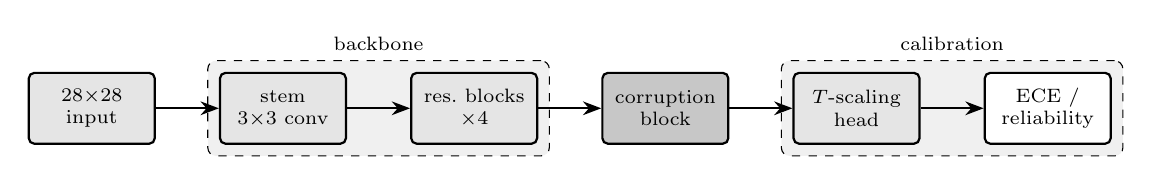
\begin{tikzpicture}[
    node distance=6mm and 8mm,
    blk/.style={draw=black, thick, rounded corners=2pt, minimum height=9mm,
      minimum width=16mm, font=\scriptsize, align=center, fill=white},
    arr/.style={-Stealth, thick, draw=black},
    grp/.style={draw=black, dashed, rounded corners=3pt, inner sep=4pt, fill=black!6}
  ]
    \node[blk, fill=black!10] (in) {28$\times$28\\input};
    \node[blk, fill=black!10, right=of in] (stem) {stem\\3$\times$3 conv};
    \node[blk, fill=black!10, right=of stem] (res) {res.\ blocks\\$\times$4};
    \node[blk, fill=black!22, right=of res] (corr) {corruption\\block};
    \node[blk, fill=black!10, right=of corr] (cal) {$T$-scaling\\head};
    \node[blk, right=of cal] (out) {ECE /\\reliability};
    \draw[arr] (in) -- (stem);
    \draw[arr] (stem) -- (res);
    \draw[arr] (res) -- (corr);
    \draw[arr] (corr) -- (cal);
    \draw[arr] (cal) -- (out);
    \begin{scope}[on background layer]
      \node[grp, fit=(stem) (res), label={[font=\scriptsize]above:backbone}] {};
      \node[grp, fit=(cal) (out), label={[font=\scriptsize]above:calibration}] {};
    \end{scope}
  \end{tikzpicture}
  \caption{Evaluation pipeline, drawn for black-and-white print. Backbone stages sit left, the corruption block is shaded darker, and the calibration head sits right of it.}
  \label{fig:pipeline}
\end{figure}

\section{Results}
\subsection{Clean Performance and Loss Comparison}
Table~\ref{tab:clean} gives the headline numbers, with three-seed means wherever we have them. Blood accuracy sits between 96.4\% and 96.8\% for every loss and every seed, a spread that falls inside binomial noise: the test set of $n=3{,}421$ gives $\pm0.3$ points at this accuracy and the validation set of $n=1{,}712$ gives $\pm0.5$. No accuracy difference below half a point is claimed anywhere in this paper. The losses separate on calibration rather than accuracy. Before scaling, raw ECE averages 1.9\% for cross-entropy, 1.3\% for focal and 0.7\% for dual-focal. After scaling, all three land near 0.7\%, with fitted temperatures of 1.6--1.7 for cross-entropy against 0.8--0.9 for the focal family. Read plainly, dual-focal needs scaling least, and scaling removes most of the difference between them. A cross-entropy baseline given the same treatment matches dual-focal after the fact, so whatever advantage the loss confers sits before scaling rather than after it.

Derma, where scaling does the most work, was run at a single seed (Table~\ref{tab:clean}). Raw ECE of 4.8\% (CE), 7.4\% (focal) and 7.4\% (dual-focal) falls to 2.0\%, 4.1\% and 2.0\% at fitted temperatures of 1.23, 1.52 and 0.77, while accuracy is unchanged by construction. The 76.5\% headline overstates how useful the model would be. Macro-F1 is 0.50 and balanced accuracy 0.49, with melanoma recall at 21.5\% (48 of 223) and dermatofibroma at 4.3\% (1 of 23) against 93.7\% for nevi. AUROC remains high at 0.93, so ranking survives even where the decisions do not. Bootstrap 95\% intervals on test accuracy run $\pm0.6$ points for blood and $\pm1.9$ for derma.

The reliability diagrams in Figures~\ref{fig:blood-rel} and \ref{fig:derma-rel} show where the clean calibration comes from. On blood, 86\% of test predictions fall in one top bin at 0.99 confidence where accuracy is 99.3\%, so the small clean ECE rests largely on a single well-behaved bin. The remaining 483 predictions spread below 0.9 confidence and follow the diagonal closely, apart from a 32-sample bin at 0.50 confidence where accuracy is 41\%. Nothing is predicted below 0.29 confidence. On derma the mass is spread across twelve bins holding 126 to 185 predictions each, and every one of them lies within 3 points of the diagonal; the two bins below 100 predictions sit 2 and 8 points low. The one conspicuous feature is a spike at 0.25 confidence with accuracy 1.0, drawn from two predictions, and its grey bar shows how little rides on it. Mean confidence tracks accuracy on both sets (0.96 blood, 0.75 derma), and classwise ECE stays low (0.004 blood, 0.019 derma), which places the residual miscalibration in the top-label confidence rather than across the whole distribution.

\begin{figure}[H]
  \centering
  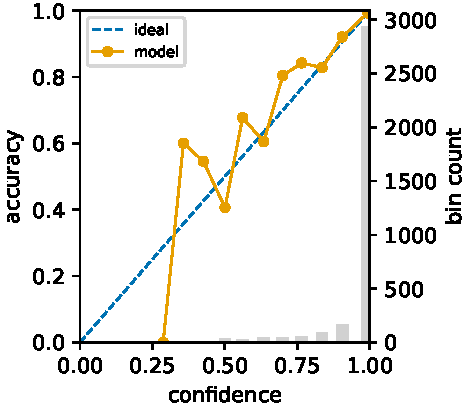
\includegraphics[width=0.7\linewidth]{fig/blood-results.reliability.pdf}
  \caption{Reliability on clean BloodMNIST test data after temperature scaling. One bin at 0.99 confidence holds 86\% of predictions and is 99.3\% accurate; below 0.9 confidence the curve tracks the diagonal apart from a 32-sample dip at 0.50 confidence. Grey bars give bin counts.}
  \label{fig:blood-rel}
\end{figure}

\begin{figure}[H]
  \centering
  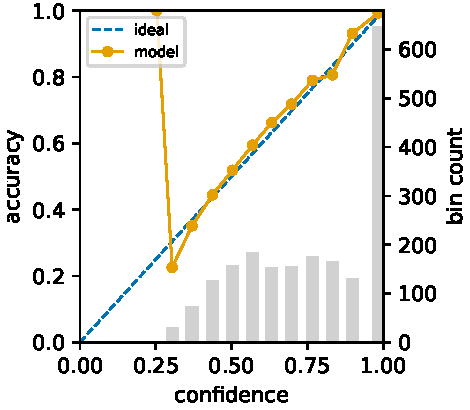
\includegraphics[width=0.7\linewidth]{fig/derma-results.reliability.pdf}
  \caption{Reliability on clean DermaMNIST test data after temperature scaling. Twelve bins of 126--185 predictions each lie within 3 points of the diagonal. The spike at 0.25 confidence comes from two predictions and carries almost no weight.}
  \label{fig:derma-rel}
\end{figure}
\subsection{Corrupted Accuracy}
Blood accuracy spreads widely across the suite (Table~\ref{tab:blood-acc}, Figure~\ref{fig:blood-acc}). Gaussian noise is survivable through severity 3, reading 96.3\%, 95.8\% and 90.9\%, and only then falls to 67.1\% and 36.3\%. Shot noise breaks the model immediately: 44.2\% at severity 1. Blur, brightness and contrast decay smoothly rather than abruptly. Pixelation and JPEG both hold above 90\% through severity 4, with JPEG at exactly 90.0\% there before dropping to 62.4\% at severity 5; pixelation is weaker at the same point, 84.9\%, so the tolerance to compression is a JPEG result rather than a general one.

\begin{figure}[H]
  \centering
  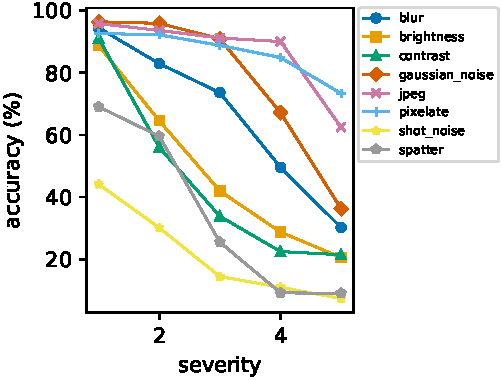
\includegraphics[width=0.7\linewidth]{fig/blood-results.severity_acc.pdf}
  \caption{BloodMNIST accuracy in percent across corruption severities 1--5. Shot noise falls from severity 1 onwards, while JPEG and pixelation hold until the later severities.}
  \label{fig:blood-acc}
\end{figure}

\begin{figure}[H]
  \centering
  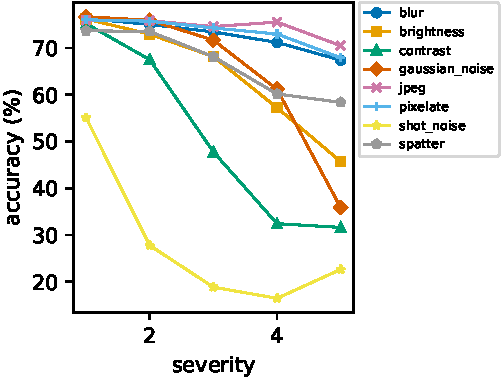
\includegraphics[width=0.7\linewidth]{fig/derma-results.severity_acc.pdf}
  \caption{DermaMNIST accuracy in percent across corruption severities 1--5. Blur, pixelation and JPEG decay slowly; contrast falls away from severity 3.}
  \label{fig:derma-acc}
\end{figure}

Derma degrades more gracefully, which is what a lower baseline invites (Table~\ref{tab:derma-acc}, Figure~\ref{fig:derma-acc}). Blur costs 8.9 points across the full range and JPEG 5.4. Brightness and contrast do far more damage, ending at 45.7\% and 31.6\% at severity 5 from clean values of 76.2\% and 75.2\%. Several of the steadier cells sit close to the 66.9\% majority-class floor, and we read those as floor effects rather than as robustness.
\subsection{Corrupted Calibration}
ECE follows accuracy down with a delay (Tables~\ref{tab:blood-ece} and \ref{tab:derma-ece}, Figures~\ref{fig:blood-sev} and \ref{fig:derma-sev}). Blood Gaussian ECE runs 2.2\%, 18.2\% and 49.2\% across severities 3 to 5. Shot noise opens at 39.1\% ECE and 44.2\% accuracy at severity 1, so the model is already confident and already wrong at the first step. Brightness ECE peaks at 48.0\% at severity 4 and then eases to 46.7\%; the reversal is small and sits inside noise-draw variance, since each image receives a single realisation with no resampling. Derma shot noise peaks at 39.7\% at severity 3 and falls back to 24.6\% as the predictions spread towards uniform wrongness. Spatter behaves differently on the two sets. Under area-scaled densities, blood ECE climbs from 22.0\% at severity 1 to 90.9\% at severity 5, whereas derma stays between 2.5\% and 5.0\% throughout because the damage pushes predictions onto the majority class without making them confident about it. Averaged over the suite, severity-5 accuracy is 0.33 on blood and 0.50 on derma, or 0.36 and 0.49 once the spatter arm is set aside.

\begin{figure}[H]
  \centering
  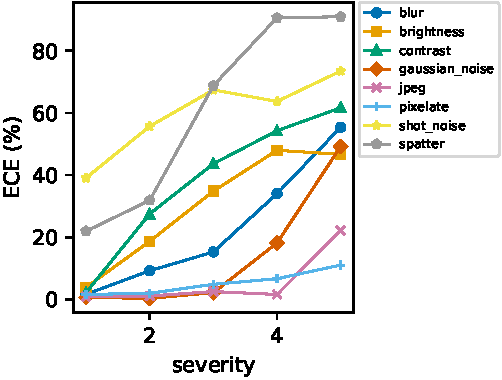
\includegraphics[width=0.7\linewidth]{fig/blood-results.severity_ece.pdf}
  \caption{BloodMNIST expected calibration error in percent across corruption severities 1--5. Spatter climbs from severity 1 to the top of the range, shot noise climbs steeply from severity 1, JPEG stays low until severity 4 and then jumps, and pixelation stays nearly flat.}
  \label{fig:blood-sev}
\end{figure}

\begin{figure}[H]
  \centering
  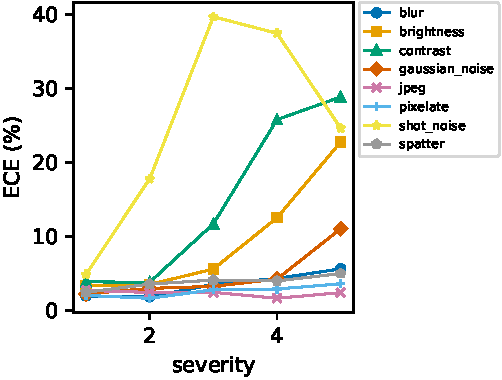
\includegraphics[width=0.7\linewidth]{fig/derma-results.severity_ece.pdf}
  \caption{DermaMNIST expected calibration error in percent across corruption severities 1--5. Shot noise peaks at severity 3 then falls, spatter stays between 2.5\% and 5.0\% throughout, contrast climbs late, and blur, pixelation and JPEG hold nearly flat.}
  \label{fig:derma-sev}
\end{figure}
\subsection{Likelihood, Brier and Confidence}
NLL and Brier add the texture that ECE cannot (Tables~\ref{tab:blood-nll} to \ref{tab:derma-brier}). Blood NLL sits at 0.11 clean and passes 30 under shot noise by severity 5. Brier climbs from 0.06 to 1.58 along the same path, and values above 1.0 are legal for an eight-class problem. Pixelation is the interesting case: accuracy barely moves between clean and severity 1, 92.6\% against 96.4\%, yet NLL doubles from 0.12 to 0.23 and Brier from 0.06 to 0.11. The degradation is visible in the likelihood scores long before it is visible in the predictions. JPEG and pixelation keep both scores comparatively flat through severity 4 on both datasets. Derma NLL starts at 0.65 with a worst corrupted cell of 3.12, an order of magnitude below blood's worst, because derma confidences never reach blood's extremes.
\subsection{Reliability under Corruption}
The clean diagrams track the diagonal apart from the sparse low-confidence bins noted earlier, and the grey bars make the empty bins legible as empty (Figures~\ref{fig:blood-rel} and \ref{fig:derma-rel}). Corruption changes the shape rather than the calibration quality. Under shot noise at severity 3 the blood curve inverts (Figure~\ref{fig:blood-shot}): accuracy stays between 9.6\% and 18.2\% in every populated bin while confidence climbs from 0.32 to 0.98, and the largest bin of all, 1,387 predictions at 0.98 confidence, is 15.8\% accurate. Derma fails differently (Figure~\ref{fig:derma-shot}). Its accuracy falls as confidence rises, from 32.9\% at 0.44 confidence to 5.7\% at 0.76, then recovers to 33.3\% in a final bin holding three predictions. Wrong answers with rising confidence on one set, falling confidence on the other, but no usable confidence on either.
\subsection{Computation}
One blood epoch took about fourteen seconds on a T4 and one derma epoch about eight. Evaluating all eight corruptions at five severities is inference only and costs under three minutes per dataset. Fitting the temperature takes seconds on CPU. The smoke-test configurations run the entire pipeline on synthetic data in under two minutes and download nothing.

\section{Discussion}
Two patterns carry practical weight. Accuracy and confidence fail at different speeds under the same corruption, so reporting one without the other hides the risk. The cheap corruptions are cheap: pixelation and JPEG at the severities typical of routine transfer pipelines cost little, which says nothing about DICOM or JPEG2000 at full resolution, since those were not tested. Brightness 1.08 and contrast 0.92 already cost blood 5 to 8 points, and that is a training artefact rather than a finding. Horizontal flips are the only augmentation in the protocol, and a model trained that way has no reason to be invariant to photometric shift. Blood's extra brittleness relative to derma plausibly traces to its dependence on stain colour, though we offer that as a hypothesis: we ran no saliency analysis to support it.

We propose no mitigation here. The natural comparisons are ensembles \parencite{lakshminarayanan2017}, MC dropout \parencite{gal2016} and stronger augmentation \parencite{ovadia2019}, all left for future work. Class-conditioned metrics with adaptive bins would harden the evaluation itself \parencite{nixon2019}, and a calibrator with a measurable error bound would strengthen claims made on small samples \parencite{kumar2019}. Ovadia and colleagues show that post-hoc scaling fades under strong shift \parencite{ovadia2019}, which bounds every claim here to the severities actually measured.

\section{Conclusion}
Compact networks reach 96.6\% accuracy on blood and 76.5\% on derma with clean ECE under 2\% after temperature scaling, measured over three seeds on blood. Corruption undoes the two unevenly. Shot noise breaks blood at severity 1 with confidence intact, JPEG and pixelation cost little until the later severities, and spatter at $28\times28$ destroys the image rather than testing the model. Dual-focal halves raw ECE against cross-entropy, and temperature scaling closes most of what remains. On the imbalanced dataset, macro-F1 of 0.50 against 76.5\% accuracy is the reason accuracy alone will not do. Every number comes from fixed-seed public runs that reproduce in minutes.

\section*{Limitations}
Resolution is $28\times28$ throughout. Larger MedMNIST+ versions exist, so whether these results transfer upward is untested. Derma runs a single seed, and every corrupted cell uses one noise realisation per image with seeds shared across corruption types. We compare no ensembles, no dropout, no augmentation schedules and no recalibration on corrupted validation data. Spatter densities scale by image area in the code used for these results; Appendix~\ref{app:spatter} records what the earlier unscaled densities did.

\section*{Declarations}
Data: BloodMNIST (CC BY 4.0) and DermaMNIST via HAM10000 (CC BY-NC 4.0, research use only). Code and checkpoints: \url{https://github.com/xmadmaxdx/medmnist-c-cal}. No funding was received.

\section*{Conflicts of Interest}
The author declares no conflicts of interest.

\appendix
\section{Implementation Details}
ResNet-18 adapted for $28\times28$ inputs (11.17M parameters), SimpleCNN three-block (0.14M), MobileNetV3-Small available (1.53M, untrained). AdamW \parencite{loshchilov2019} at $10^{-3}$, weight decay $5\times10^{-4}$, batch 128, twenty epochs, StepLR halving every six epochs, seed 0--2 blood ResNet and seed 0 elsewhere, Colab T4, PyTorch. Temperature fitted on validation logits only. Corruption seeds equal the sample index.
\section{Spatter Forensics}
\label{app:spatter}
Mean pixel values of a random frame under the original spatter severities 1--5 read 72.9, 11.1, 0.8, 0.0 and 0.0 on the 0--255 scale. From severity 3 the frames were pure black, so the identical metric rows first reported reflected identical inputs rather than model behaviour. Densities built for 224-pixel images must scale by image area, a factor of $1/64$ at $28\times28$, before reuse, and the code used for this paper does so. All spatter rows in the tables above follow the scaled protocol: blood accuracy degrades 69.0\%, 59.6\%, 25.5\%, 9.2\% and 9.1\% instead of sitting flat, while derma tolerates the same damage from 73.7\% down to 58.4\%. Even scaled, blobs of radius up to 11 pixels cover a large fraction of a 28-pixel frame, so spatter remains the harshest occlusion test in the suite rather than a fair one.

Twelve tables follow, collecting every number the main text cites. Tables~1 and~2 fix the datasets and corruption parameters so the damage can be reproduced exactly. Table~3 summarises the trained matrix by validation accuracy with seed means. Tables~4 to~12 give the per-severity results for both datasets: accuracy, calibration error, likelihood and Brier score. Spatter rows are retained throughout, including where the inputs degenerate as diagnosed above.

\begin{table}[H]
  \centering
  \caption{Dataset summary. Fixed public splits throughout.}
  \label{tab:data}
  \begin{tabular}{lcccc}
    \toprule
    Set & Classes & Train & Val & Test \\
    \midrule
    BloodMNIST & 8 & 11,959 & 1,712 & 3,421 \\
    DermaMNIST & 7 & 7,007 & 1,003 & 2,005 \\
    \bottomrule
  \end{tabular}
\end{table}

\begin{table}[H]
  \centering
  \caption{Corruption parameters per severity 1--5 on 0--255 uint8 images before normalisation. Seeds equal the sample index.}
  \label{tab:corr}
  \begin{tabular}{lccccc}
    \toprule
    Corruption & S1 & S2 & S3 & S4 & S5 \\
    \midrule
    Gaussian noise $\sigma$ & 2.0 & 6.0 & 12.0 & 20.0 & 30.0 \\
    Shot noise $\lambda$ & 60 & 25 & 12 & 6 & 3 \\
    Blur radius (px) & 0.4 & 0.8 & 1.2 & 1.8 & 2.5 \\
    Brightness factor & 1.08 & 1.18 & 1.32 & 1.50 & 1.70 \\
    Contrast factor & 0.92 & 0.80 & 0.65 & 0.50 & 0.35 \\
    Pixelate scale & 0.85 & 0.70 & 0.55 & 0.40 & 0.30 \\
    JPEG quality & 85 & 65 & 45 & 28 & 12 \\
    Spatter blobs & 30 & 80 & 160 & 300 & 500 \\
    \bottomrule
  \end{tabular}
\end{table}

\begin{table}[H]
  \centering
  \caption{Best validation accuracy (\%) on BloodMNIST with seed means. Corrupted evaluation per arm uses the same protocol throughout.}
  \label{tab:val}
  \begin{tabular}{lcccc}
    \toprule
    Backbone & CE & Focal & Dual-focal \\
    \midrule
    ResNet-18 & 96.64 $\pm$ 0.21 & 96.72 $\pm$ 0.14 & 96.58 $\pm$ 0.09 \\
    SimpleCNN & 96.55 & 96.96 & 96.85 \\
    \bottomrule
  \end{tabular}
\end{table}

\begin{table}[H]
  \centering
  \caption{Clean test performance after temperature scaling. Raw ECE before scaling in parentheses.}
  \label{tab:clean}
  \begin{tabular}{lcccccc}
    \toprule
    Set & Loss & Acc.\ (\%) & ECE (\%) & NLL & Brier & $T$ \\
    \midrule
    Blood & CE & 96.6 & 0.7 (1.9) & 0.11 & 0.05 & 1.66 \\
    Blood & Focal & 96.5 & 0.7 (1.3) & 0.11 & 0.05 & 0.86 \\
    Blood & Dual & 96.5 & 0.7 (0.7) & 0.12 & 0.05 & 0.90 \\
    Derma & CE & 75.4 & 2.0 (4.8) & 0.65 & 0.33 & 1.23 \\
    Derma & Focal & 75.8 & 4.1 (7.4) & 0.67 & 0.33 & 1.52 \\
    Derma & Dual & 76.5 & 2.0 (7.4) & 0.65 & 0.33 & 0.77 \\
    \bottomrule
  \end{tabular}
\end{table}

\begin{table}[H]
  \centering
  \caption{BloodMNIST accuracy (\%) per corruption and severity, dual-focal ResNet-18.}
  \label{tab:blood-acc}
  \begin{tabular}{lccccc}
    \toprule
    Corruption & S1 & S2 & S3 & S4 & S5 \\
    \midrule
    Gaussian noise & 96.3 & 95.8 & 90.9 & 67.1 & 36.3 \\
    Shot noise & 44.2 & 30.2 & 14.5 & 11.0 & 7.4 \\
    Blur & 94.4 & 82.9 & 73.6 & 49.6 & 30.2 \\
    Brightness & 88.7 & 64.5 & 42.0 & 28.8 & 20.6 \\
    Contrast & 91.1 & 56.0 & 33.8 & 22.5 & 21.5 \\
    Pixelate & 92.6 & 92.2 & 88.8 & 84.9 & 73.3 \\
    JPEG & 95.8 & 93.6 & 91.1 & 90.0 & 62.4 \\
    Spatter & 69.0 & 59.6 & 25.5 & 9.2 & 9.1 \\
    \bottomrule
  \end{tabular}
\end{table}

\begin{table}[H]
  \centering
  \caption{BloodMNIST ECE (\%) per corruption and severity. Clean ECE is 0.7\%.}
  \label{tab:blood-ece}
  \begin{tabular}{lccccc}
    \toprule
    Corruption & S1 & S2 & S3 & S4 & S5 \\
    \midrule
    Gaussian noise & 0.6 & 0.4 & 2.2 & 18.2 & 49.2 \\
    Shot noise & 39.1 & 55.7 & 67.4 & 63.7 & 73.5 \\
    Blur & 1.7 & 9.2 & 15.3 & 34.0 & 55.4 \\
    Brightness & 3.9 & 18.7 & 34.8 & 48.0 & 46.7 \\
    Contrast & 2.2 & 27.5 & 43.6 & 54.3 & 61.7 \\
    Pixelate & 1.6 & 2.0 & 4.9 & 6.7 & 11.1 \\
    JPEG & 0.9 & 1.1 & 2.5 & 1.6 & 22.2 \\
    Spatter & 22.0 & 31.9 & 68.8 & 90.6 & 90.9 \\
    \bottomrule
  \end{tabular}
\end{table}

\begin{table}[H]
  \centering
  \caption{DermaMNIST accuracy (\%) per corruption and severity, dual-focal ResNet-18.}
  \label{tab:derma-acc}
  \begin{tabular}{lccccc}
    \toprule
    Corruption & S1 & S2 & S3 & S4 & S5 \\
    \midrule
    Gaussian noise & 76.7 & 75.9 & 71.7 & 61.1 & 35.9 \\
    Shot noise & 55.1 & 27.8 & 18.9 & 16.5 & 22.6 \\
    Blur & 76.3 & 75.0 & 73.4 & 71.2 & 67.4 \\
    Brightness & 76.2 & 72.9 & 68.1 & 57.2 & 45.7 \\
    Contrast & 75.2 & 67.5 & 47.8 & 32.4 & 31.6 \\
    Pixelate & 76.0 & 75.7 & 74.3 & 73.0 & 67.9 \\
    JPEG & 75.9 & 75.8 & 74.6 & 75.5 & 70.5 \\
    Spatter & 73.7 & 73.5 & 68.1 & 60.2 & 58.4 \\
    \bottomrule
  \end{tabular}
\end{table}

\begin{table}[H]
  \centering
  \caption{DermaMNIST ECE (\%) per corruption and severity. Clean ECE is 2.0\%.}
  \label{tab:derma-ece}
  \begin{tabular}{lccccc}
    \toprule
    Corruption & S1 & S2 & S3 & S4 & S5 \\
    \midrule
    Gaussian noise & 2.2 & 3.0 & 3.2 & 4.2 & 11.0 \\
    Shot noise & 4.9 & 17.8 & 39.7 & 37.5 & 24.6 \\
    Blur & 2.0 & 1.8 & 3.5 & 4.3 & 5.6 \\
    Brightness & 3.3 & 3.5 & 5.6 & 12.5 & 22.8 \\
    Contrast & 3.9 & 3.8 & 11.7 & 25.8 & 28.9 \\
    Pixelate & 2.0 & 1.6 & 2.8 & 2.9 & 3.6 \\
    JPEG & 2.7 & 2.4 & 2.4 & 1.6 & 2.4 \\
    Spatter & 2.5 & 3.6 & 4.1 & 4.0 & 5.0 \\
    \bottomrule
  \end{tabular}
\end{table}

\begin{table}[H]
  \centering
  \caption{BloodMNIST NLL per corruption and severity. Clean NLL is 0.12.}
  \label{tab:blood-nll}
  \begin{tabular}{lccccc}
    \toprule
    Corruption & S1 & S2 & S3 & S4 & S5 \\
    \midrule
    Gaussian noise & 0.12 & 0.13 & 0.27 & 1.22 & 3.53 \\
    Shot noise & 2.42 & 4.61 & 7.36 & 16.86 & 34.82 \\
    Blur & 0.18 & 0.62 & 1.25 & 2.55 & 4.03 \\
    Brightness & 0.35 & 1.21 & 2.80 & 4.81 & 5.93 \\
    Contrast & 0.28 & 2.02 & 3.83 & 4.20 & 4.48 \\
    Pixelate & 0.23 & 0.24 & 0.45 & 0.54 & 1.03 \\
    JPEG & 0.14 & 0.19 & 0.28 & 0.31 & 1.33 \\
    Spatter & 2.35 & 4.04 & 13.06 & 39.35 & 64.46 \\
    \bottomrule
  \end{tabular}
\end{table}

\begin{table}[H]
  \centering
  \caption{BloodMNIST Brier score per corruption and severity. Clean Brier is 0.06. Range is 0 to 2 for eight classes.}
  \label{tab:blood-brier}
  \begin{tabular}{lccccc}
    \toprule
    Corruption & S1 & S2 & S3 & S4 & S5 \\
    \midrule
    Gaussian noise & 0.06 & 0.06 & 0.13 & 0.51 & 1.08 \\
    Shot noise & 0.89 & 1.20 & 1.45 & 1.44 & 1.58 \\
    Blur & 0.09 & 0.27 & 0.44 & 0.81 & 1.18 \\
    Brightness & 0.17 & 0.51 & 0.86 & 1.11 & 1.18 \\
    Contrast & 0.13 & 0.71 & 1.11 & 1.25 & 1.35 \\
    Pixelate & 0.11 & 0.12 & 0.18 & 0.23 & 0.40 \\
    JPEG & 0.07 & 0.09 & 0.14 & 0.15 & 0.57 \\
    Spatter & 0.54 & 0.72 & 1.42 & 1.81 & 1.82 \\
    \bottomrule
  \end{tabular}
\end{table}

\begin{table}[H]
  \centering
  \caption{DermaMNIST NLL per corruption and severity. Clean NLL is 0.65.}
  \label{tab:derma-nll}
  \begin{tabular}{lccccc}
    \toprule
    Corruption & S1 & S2 & S3 & S4 & S5 \\
    \midrule
    Gaussian noise & 0.65 & 0.67 & 0.76 & 1.02 & 1.46 \\
    Shot noise & 1.15 & 1.58 & 2.08 & 2.61 & 3.12 \\
    Blur & 0.65 & 0.68 & 0.73 & 0.82 & 0.93 \\
    Brightness & 0.66 & 0.74 & 0.91 & 1.19 & 1.49 \\
    Contrast & 0.68 & 0.85 & 1.23 & 1.57 & 1.68 \\
    Pixelate & 0.67 & 0.67 & 0.70 & 0.72 & 0.84 \\
    JPEG & 0.65 & 0.66 & 0.69 & 0.69 & 0.82 \\
    Spatter & 0.72 & 0.74 & 0.91 & 1.29 & 1.52 \\
    \bottomrule
  \end{tabular}
\end{table}

\begin{table}[H]
  \centering
  \caption{DermaMNIST Brier score per corruption and severity. Clean Brier is 0.33. Range is 0 to 2 for seven classes.}
  \label{tab:derma-brier}
  \begin{tabular}{lccccc}
    \toprule
    Corruption & S1 & S2 & S3 & S4 & S5 \\
    \midrule
    Gaussian noise & 0.33 & 0.34 & 0.39 & 0.51 & 0.73 \\
    Shot noise & 0.57 & 0.78 & 1.00 & 1.01 & 0.87 \\
    Blur & 0.33 & 0.35 & 0.37 & 0.40 & 0.44 \\
    Brightness & 0.34 & 0.37 & 0.44 & 0.58 & 0.74 \\
    Contrast & 0.35 & 0.44 & 0.65 & 0.81 & 0.82 \\
    Pixelate & 0.34 & 0.34 & 0.35 & 0.37 & 0.42 \\
    JPEG & 0.33 & 0.34 & 0.35 & 0.35 & 0.40 \\
    Spatter & 0.36 & 0.36 & 0.43 & 0.54 & 0.58 \\
    \bottomrule
  \end{tabular}
\end{table}

\begin{figure}[H]
  \centering
  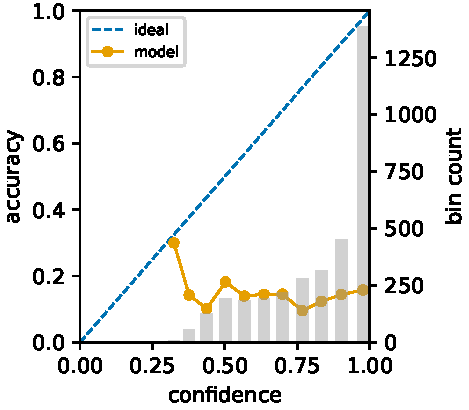
\includegraphics[width=0.7\linewidth]{fig/blood-shot-sev3.pdf}
  \caption{Reliability under shot noise at severity 3 on BloodMNIST. Accuracy sits between 9.6\% and 18.2\% in every populated bin while confidence rises from 0.32 to 0.98; the largest bin, 1,387 predictions at 0.98 confidence, is 15.8\% accurate.}
  \label{fig:blood-shot}
\end{figure}

\begin{figure}[H]
  \centering
  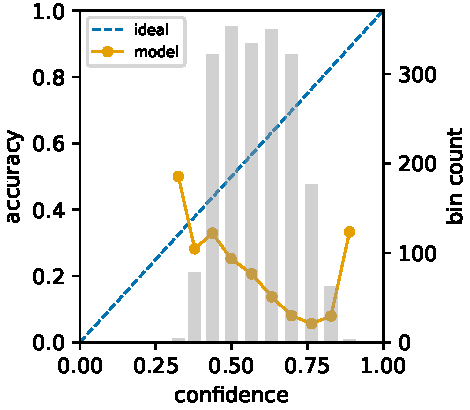
\includegraphics[width=0.7\linewidth]{fig/derma-shot-sev3.pdf}
  \caption{Reliability under shot noise at severity 3 on DermaMNIST. Accuracy falls as confidence rises, from 32.9\% at 0.44 confidence to 5.7\% at 0.76, then recovers to 33.3\% in a final bin holding three predictions.}
  \label{fig:derma-shot}
\end{figure}

\section*{Bibliography}
\printbibliography[heading=none]

\end{document}
